\documentclass[border=12pt]{standalone}
\usepackage[utf8]{inputenc}
\usepackage[utf8]{vietnam}
\usepackage{amsmath,amsfonts,amssymb}
\usepackage{siunitx}
\usepackage{tikz}
\usetikzlibrary{arrows, decorations.markings, calc, fadings, decorations.pathreplacing, patterns, decorations.pathmorphing, positioning}
\begin{document}
	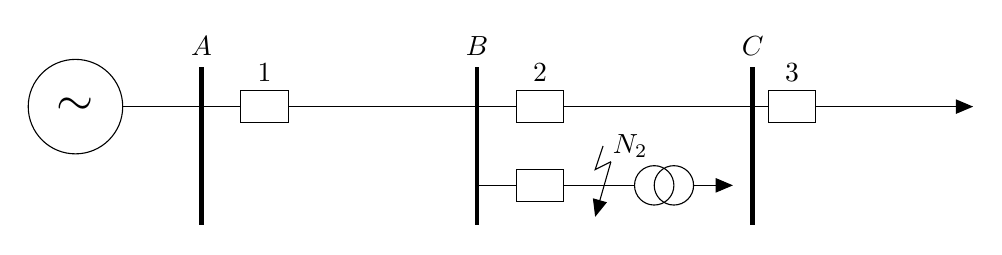
\begin{tikzpicture}[>=triangle 45]
		\draw (-.1,0) circle (.6)  node{\LARGE{$\mathbf{\sim}$}};
		\draw (0.5, 0) -- (1.5,0);
		
		\draw[ultra thick] (1.5,.5) node[above]{$A$} -- (1.5, -1.5);
		\draw (1.5,0) -- (2,0); \draw (2,0.2) rectangle (2.6,-0.2); \draw (2.3, 0.2) node[above]{$1$}; \draw (2.6,0) -- (5,0);
		
		\draw[ultra thick] (5,.5) node[above]{$B$} -- (5, -1.5);
		\draw (5,0) -- (5.5,0); \draw (5.5,0.2) rectangle (6.1,-0.2); \draw (5.8, 0.2) node[above]{$2$}; \draw (6.1,0) -- (8.5,0);
		\draw (5,-1) -- (5.5, -1); \draw (5.5,-.8) rectangle (6.1,-1.2); \draw (6.1,-1) -- (7,-1); \draw (7.25,-1) circle (0.25); \draw (7.5,-1) circle (0.25); \draw[->] (7.75, -1) -- (8.25,-1); \draw (6.6,-0.5) node[right]{$N_2$} -- (6.5,-0.8) -- (6.7, -0.7); \draw[->] (6.7, -0.7) -- (6.5,-1.4);
		
		\draw[ultra thick] (8.5,.5) node[above]{$C$} -- (8.5, -1.5);
		\draw (8.5,0) -- (8.7,0); \draw (8.7,0.2) rectangle (9.3,-0.2); \draw (9, 0.2) node[above]{$3$}; \draw[->] (9.3,0) -- (11.3,0);
	\end{tikzpicture}
\end{document} 